%%
%% crosscountry.tex -- Flight Gear documentation: The FlightGear Manual
%% Chapter file
%%
%% Written by Michael Basler, started September 1998.
%%
%% Copyright (C) 2002 Michael Basler
%%
%%
%% This program is free software; you can redistribute it and/or
%% modify it under the terms of the GNU General Public License as
%% published by the Free Software Foundation; either version 2 of the
%% License, or (at your option) any later version.
%%
%% This program is distributed in the hope that it will be useful, but
%% WITHOUT ANY WARRANTY; without even the implied warranty of
%% MERCHANTABILITY or FITNESS FOR A PARTICULAR PURPOSE.  See the GNU
%% General Public License for more details.
%%
%% You should have received a copy of the GNU General Public License
%% along with this program; if not, write to the Free Software
%% Foundation, Inc., 675 Mass Ave, Cambridge, MA 02139, USA.
%%
%% $Id: crosscountry.tex,v 0.1 2005/09/09 michael
%% (Log is kept at end of this file)

%%%%%%%%%%%%%%%%%%%%%%%%%%%%%%%%%%%%%%%%%%%%%%%%%%%%%%%%%%%%%%%%%%%%
\ifchinese
\chapter{{\\}短途转场飞行教程}
\fi
\chapter{A Cross Country Flight Tutorial}
\label{crosscountry}
%%%%%%%%%%%%%%%%%%%%%%%%%%%%%%%%%%%%%%%%%%%%%%%%%%%%%%%%%%%%%%%%%%%%

%%%%%%%%%%%%%%%%%%%%%%%%%% CHINESE VERSION %%%%%%%%%%%%%%%%%%%%%%%%%

\ifchinese
\section{简介}

\begin{figure}[!htp]
\centering
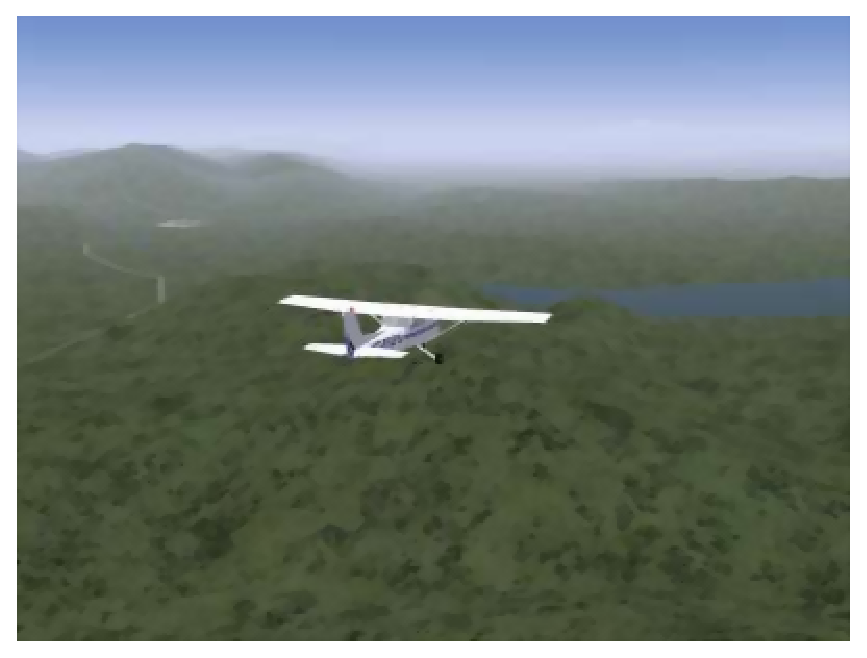
\includegraphics[width=0.5\textwidth]{antonio2}
\caption{从圣安东尼奥大坝飞到利弗莫尔}
\end{figure}

本教程将会模拟一次转场飞行,从里德—晓岚机场(Reid-Hillview,KRHV)到利弗莫尔机场(Livermore,KLVK),使用目视飞行规则(Visual Flight Rules,VFR)。这两个机场都已经包括在了 FlightGear 的基础包里,因此不需要另外安装地景。

我假设你已经学会了 FlightGear 里的起飞、爬升、转弯、下降和降落。否则,建议你看一下之前的教程。本教程基于之前的教程基础,并增加了飞行系统和程序方面更复杂的信息。

%%%%%%%%%%%%%%%%%%%%%%%%%% ENGLISH VERSION %%%%%%%%%%%%%%%%%%%%%%%%%
\iffalse
\section{Introduction}

\begin{figure}[!htp]
\centering
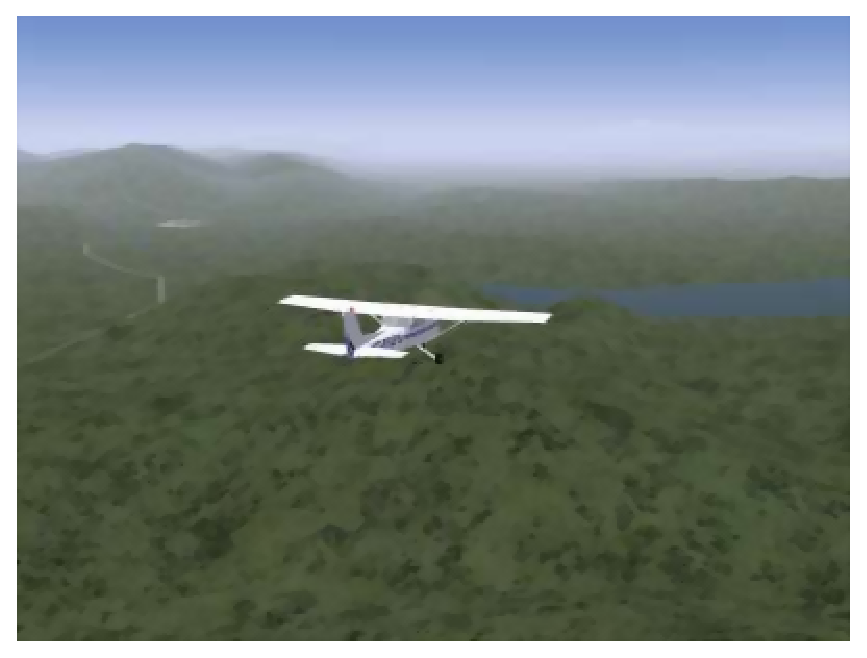
\includegraphics[width=0.5\textwidth]{antonio2}
\caption{Flying over the San Antonio Dam to Livermore}
\end{figure}

This tutorial simulates a cross-country flight from Reid-Hillview (KRHV) to
Livermore (KLVK) under Visual Flight Rules (VFR). Both airports are
included in the standard FlightGear package, so no additional scenery is required.

I'll assume that you are happy taking off, climbing, turning, descending
and landing in FlightGear. If not, have alook at the tutorials listed above.
This tutorial is designed to follow on from them and provide information on
some of the slightly more complicated flight systems and procedures.

\subsection{Disclaimer and Thanks}

A quick disclaimer. I fly microlights rather than Cessnas in real life. Most of
this information has been gleaned from various non-authoritive sources. If you
find an error or misunderstanding, please let me know. Mail me at
stuart\_d\_buchanan -at- yahoo.co.uk.

I'd like to thank the following people for helping make this tutorial accurate
and readable: Benno Schulenberg, Sid Boyce, Vassilii Khachaturov, James Briggs.

\section{Flight Planning}

Before we begin, we need to plan our flight.
Otherwise we'll be taking off not knowing whether to turn left or right.

First, have a look at the \Index{Sectional} for the area. This is a map for
flying showing airports, navigational aids, and obstructions.
There are two scales of sectionals for VFR flight -
the 1:500,000 sectionals themselves, and a number of
1:250,000 VFR Terminal Area Charts which cover particularly busy areas.

They are available from pilot shops, or on the web from various sources.
You can access a Google-map style interface here:

\medskip
\web{http://www.runwayfinder.com/}
\medskip

Simple search for Reid-Hillview. An extract from the chart is shown in Figure~\ref{sectional}.

\begin{figure}[!htp]
\centering
\includegraphics[width=\textwidth]{sectional}
\caption{Sectional extract showing Reid-Hillview and Livermore airports\label{sectional}}
\end{figure}

If you want a map of the entire area showing exactly where the plane is,
you can use Atlas.
This is a moving-map program that connects to FlightGear. See Section \ref{Atlas} for details.

So, how are we going to fly from Reid-Hillview to Livermore?

We'll be taking off from runway 31R at KRHV. KRHV is the ICAO code
for \Index{Reid-Hillview} airport, and is shown in the FlightGear wizard.
(It is marked on the sectional as RHV for historic reasons.
To get the ICAO code, simply prefix a `K'.)

The 31 indicates that the magnetic heading of the runway is around 310 degrees,
and the R indicates that it's the runway on the right. As can be seen from the
sectional, there are two parallel runways at KRHV. This is to handle the large
amount of traffic that uses the airport. Each of the runways can be used in
either direction. Runway 31 can be used from the other end as runway 13.
So, the runways available are 13R, 13L, 31R, 31L. Taking off and landing
is easier done into the wind, so when the wind is coming from the North West,
runways 31L and 31L will be in use. The name of the runway is written in large
letters at the beginning and is easily seen from the air.

Once we take off we'll head at 350 degrees magnetic towards \Index{Livermore} (KLVK).
We'll fly at about 3,500ft about sea-level. This puts us at least 500ft above any
terrain or obstructions like radio masts on the way.

We'll fly over the Calaveras Reservoir then the San Antonio Reservoir. These are
both large bodies of water and we can use them as navigation aids to ensure we
stay on the right track.

Once we get about 10 miles out of Livermore (above the San Antonia Reservoir),
we'll contact the Livermore Air Traffic Control (ATC) to find out
where we should land. We'll then join the circuit and land.

\section{Getting Up}

OK, we know where we're going and how we'll get there. Time to get started.

Start FlightGear using the Wizard (or command-line if you prefer).
 We want to use a C172P and take off from runway 31R at Reid-Hillview of
 Santa Clara County (KRHV). Dawn is a nice time to fly in California.

If you want, you can fly in the current weather at KRHV by clicking the
Advanced button on the final screen of the Wizard, selecting Weather
from the left-hand pane, selecting `Fetch real weather' and clicking OK.

\begin{figure}[!htp]
\centering
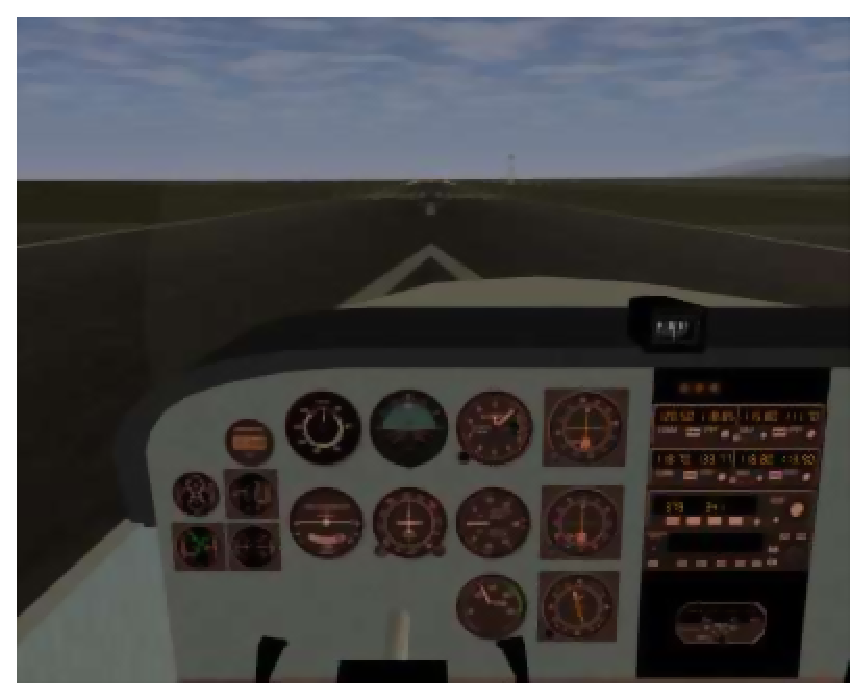
\includegraphics[width=0.5\textwidth]{krhvrunway}
\caption{On the runway at KRHV}
\end{figure}

\subsection{Pre-Flight}

Before we take off, we need to pre-flight the aircraft. In the real world,
this consists of walking around the aircraft to check nothing has fallen
off, and checking we have enough fuel.

In our case, we'll take the opportunity to check the weather, set our
altimeter and pre-set things that are easier to do when you're not flying.

The weather is obviously important when flying. We need to know if
there is any sort of cross-wind that might affect take-off, at what
altitude any clouds are (this is a VFR flight - so we need to stay
well away from clouds at all times), and any wind that might blow us off course.

We also need to calibrate our altimeter. Altimeters calculate the
current alititude indirectly by measuring air pressure, which decreases
as you ascend. However, weather systems can affect the air pressure and
lead to incorrect altimeter readings, which can be deadly if flying in mountains.

\subsection{ATIS}

Conveniently, airports broadcast the current sea-level pressure along
with useful weather and airport information over the \Index{ATIS}.
This is a recorded message that is broadcast over the radio.
However, to listen to it, we need to tune the radio to the correct frequency.

The ATIS frequency is displayed on the sectional (look for `ATIS' near the airport), but is also
available from within FlightGear. To find out the frequencies for an
airport (including the tower, ground and approach if appropriate),
use the ATC/AI menu and select Frequencies. Then enter the ICAO code
(KRHV) into the dialog box. The various frequencies associated with the
airport are then displayed. Duplicates indicate that the airport uses
multiple frequencies for that task, and you may use either.

Either way, the ATIS frequency for Reid-Hillview is 125.2MHz.

\subsection{Radios}

We now need to tune the \Index{radio}. The radio is located in the Radio
Stack to the right of the main instruments. There are actually two
independent radio systems, 1 and 2.  Each radio is split in two,
with a communications (COMM) radio on the left, and a navigation
(NAV) radio on the right. We want to tune COMM1 to the ATIS frequency.

\begin{figure}[!htp]
\centering
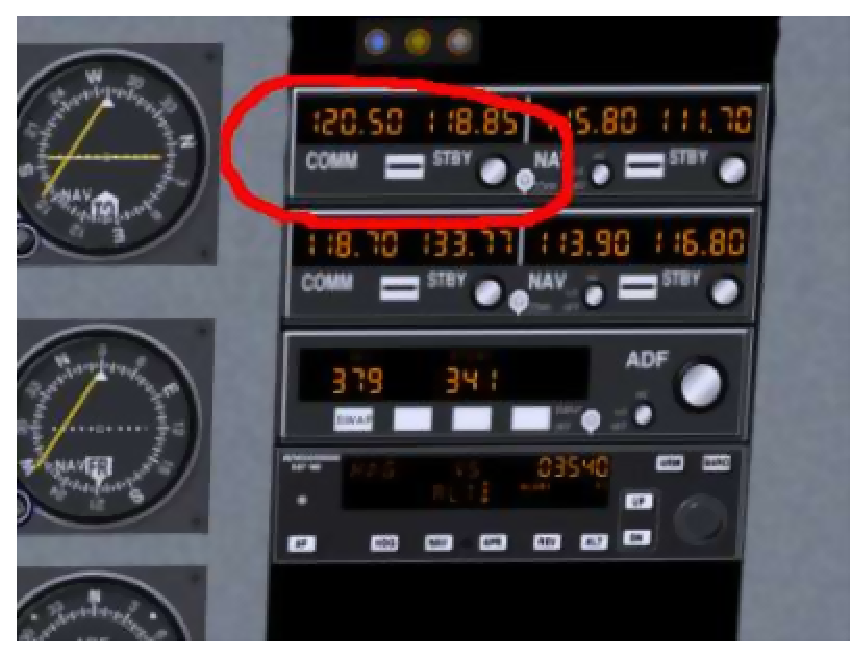
\includegraphics[width=0.5\textwidth]{comm1}
\caption{The C172 communications stack with COMM1 highlighted\label{comm1}}
\end{figure}

The radio has two frequencies, the active frequency, which is currently in use,
and the standby frequency, which we tune to the frequency we wish to use next.
The active frequency is shown on the left 5 digits, while the standby frequency
is shown on the right. We change the standby frequency, then swap the two over,
so the standby becomes active and the active standby. This way, we don't lose
radio contact while tuning the radio.

\begin{figure}[!htp]
\centering
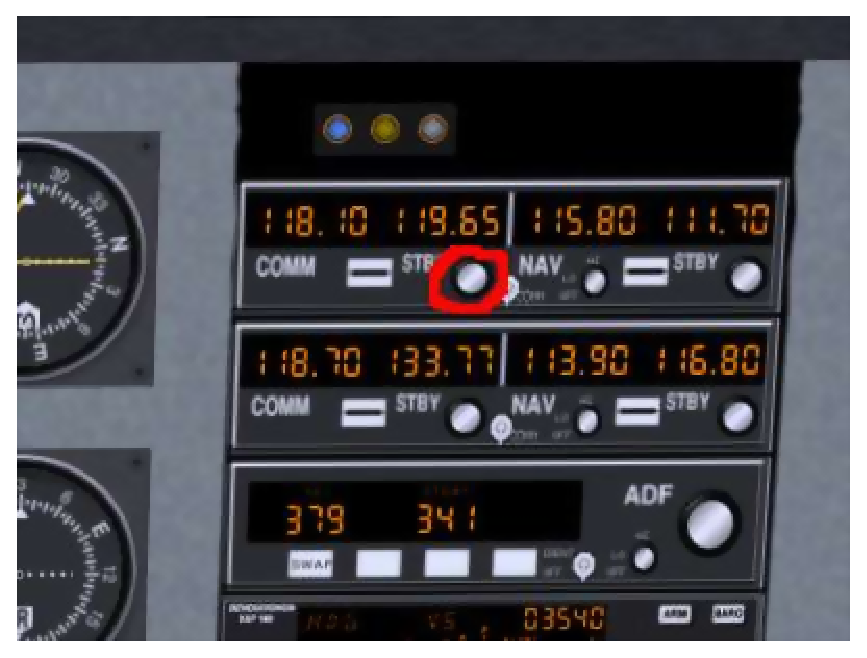
\includegraphics[width=0.5\textwidth]{comm1_knob}
\caption{COMM1 adjustment knob\label{comm1knob}}
\end{figure}

To change the frequency, click on the grey knob below the standby frequency
(highlighted in Figure~\ref{comm1knob}), just to the right of the `STBY'.
Using the left mouse button changes the number after the decimal place,
using the middle button changes the numbers before the decimal place.
Click on the right side of the button to change the frequency up, and
the left of the button to change the frequency down. Most of the FlightGear
cockpit controls work this way. If you are having difficulty clicking on the
correct place, press Ctrl-C to highlight the hot-spots for clicking.

\begin{figure}[!htp]
\centering
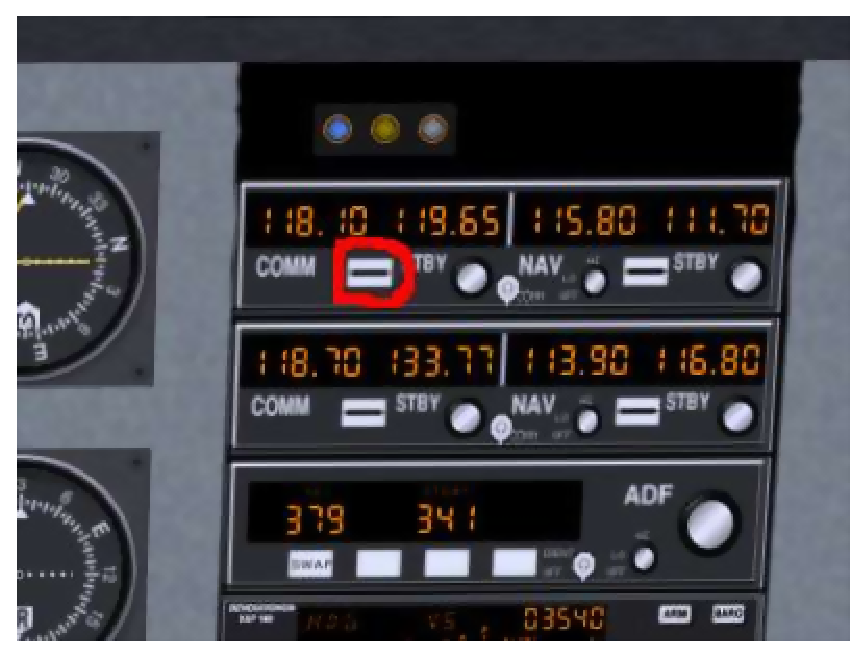
\includegraphics[width=0.5\textwidth]{comm1_switch}
\caption{COMM1 switch\label{comm1switch}}
\end{figure}

Once you have changed the frequency to 125.2, press the white button between
the words `COMM' and `STBY' to swap the active and standby frequencies
(highlighted in Figure~\ref{comm1switch}). After a second or so, you'll hear the ATIS information.

\subsection{Altimeter and Compass}

\begin{figure}[!htp]
\centering
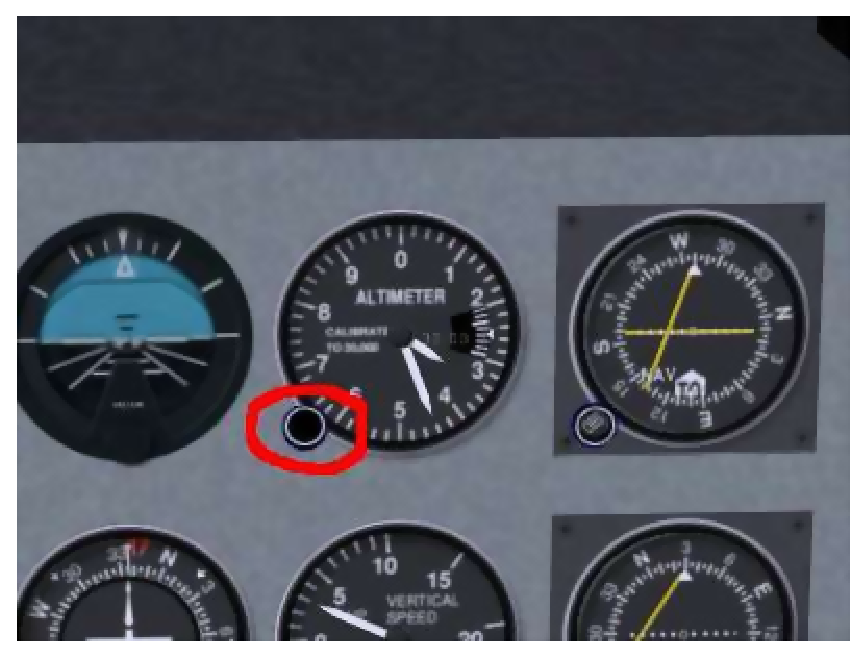
\includegraphics[width=0.5\textwidth]{altimeter}
\caption{Altimeter calibration knob\label{altimeter}}
\end{figure}

Listen for the `\Index{Altimeter}' setting. If you are not using `real weather',
the value will be 2992, which is standard and already set on the plane.
If you are using `real weather', then the altimeter value is likely to be different.
We therefore need to set the altimeter to the correct value.
To do this, use the knob at the bottom left of the altimeter
(circled in red in Figure~\ref{altimeter}), in the same way as
you changed the radio frequency. This changes the value in the
little window on the right of the altimeter, which is what you are
trying to set, as well as the altitude displayed by the altimeter.

The other way to set the altimeter is to match it to the elevation above
sea-level of the airport. The elevation is listed on the sectional.
For KRHV it is 133ft. This means you can double-check the pressure value reported over ATIS.

\begin{figure}[!htp]
\centering
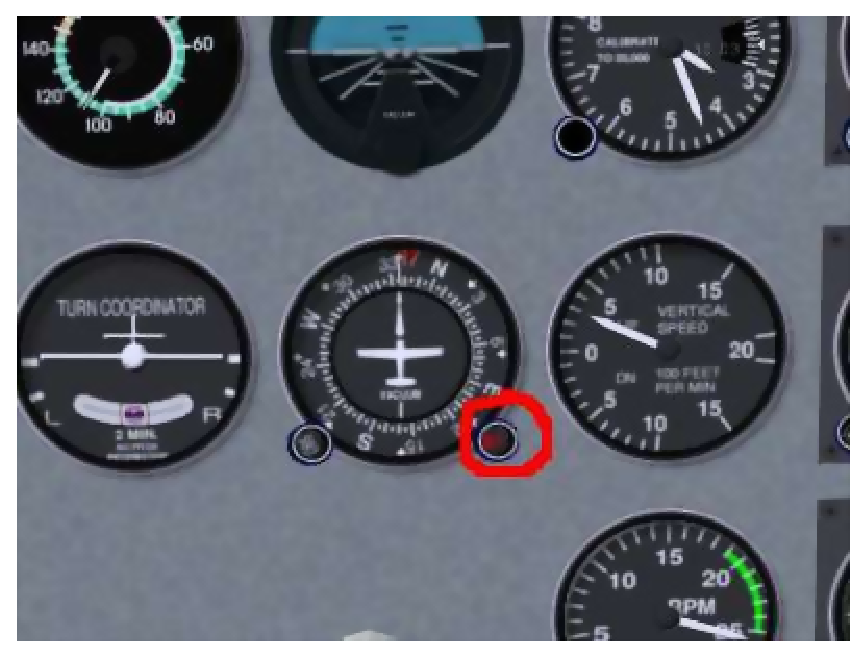
\includegraphics[width=0.5\textwidth]{compass}
\caption{Heading adjust knob\label{head}}
\end{figure}

We will also take the opportunity to set the heading bug on the compass to 350 -
our bearing from KRHV to KLVK. To do this, use the red button on the compass
housing (highlighted in Figure~\ref{head}), just as you've done before.
Use the left mouse button for small adjustments, and middle mouse button
to make big adjustments. The value of 350 is just anti-clockwise of the
labeled value of N (North - 0 degrees).

\begin{figure}[!htp]
\centering
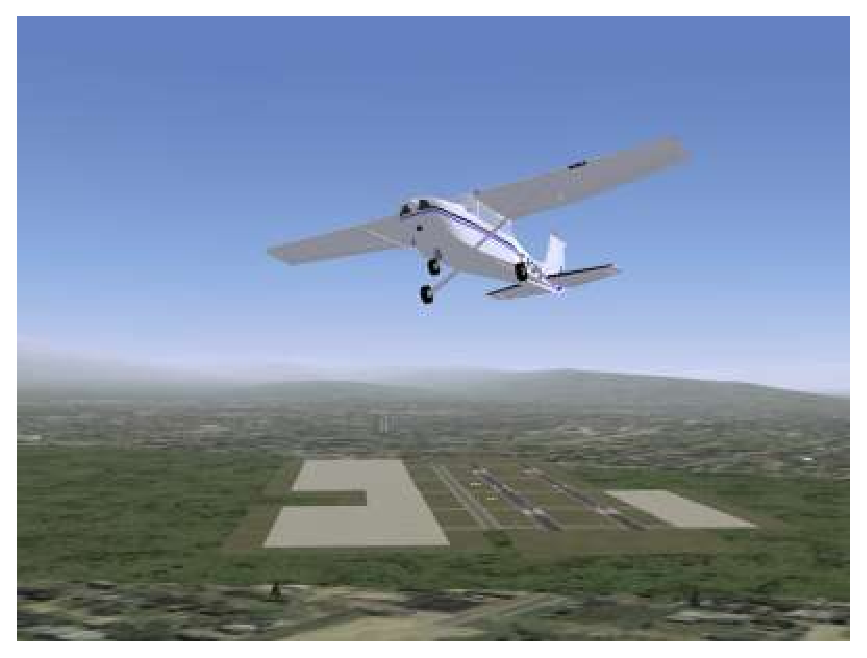
\includegraphics[width=0.5\textwidth]{takeoff}
\caption{Take-off from KRHV}
\end{figure}

\subsection{Take-Off}

OK, now we've done that we can actually take off!. In my case this usually
involves weaving all over the runway, and swerving to the left once
I've actually left the ground, but you'll probably have better control than me.
Once above 1000ft, make a gentle turn to the right to a heading of 350 degrees.
As we've set the heading bug, it will be easy to follow. We're aiming for a fairly prominent valley.


Continue climbing to 3,500 ft at around 500-700 fpm. Once you reach that altitude,
reduce power, level off to level flight and trim appropriately. Check the power
again and adjust so it's in the green arc of the RPM guage. We shouldn't run the
engine at maximum RPM except during take-off.

\section{Cruising}

OK, we've taken off and are on our way to Livermore. Now we can make our life a
bit easier by using the autopilot and our plane more fuel efficient by tuning
the engine. We'll also want to check we're on-course

\subsection{The Autopilot}

\begin{figure}[!htp]
\centering
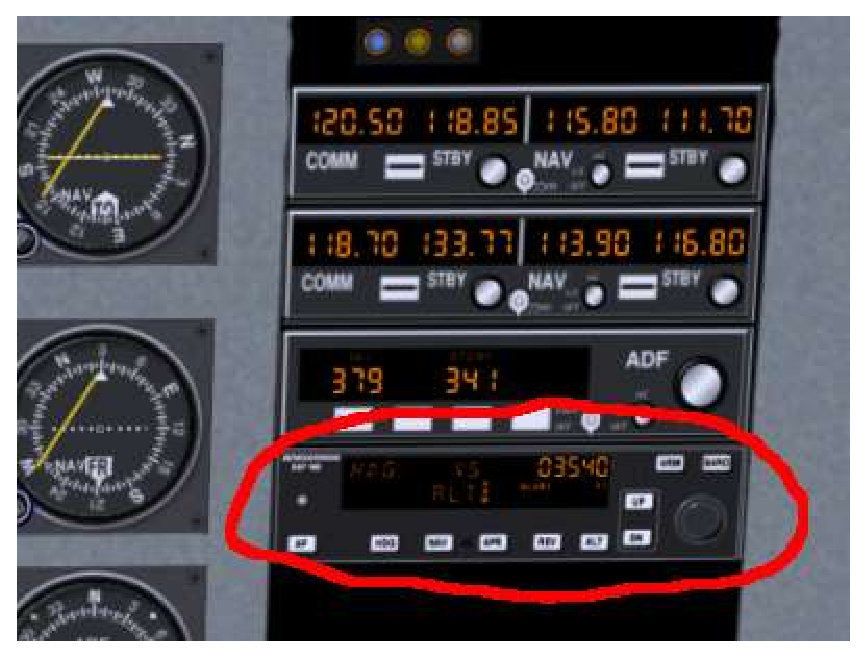
\includegraphics[width=0.5\textwidth]{autopilot}
\caption{The C172 Autopilot\label{autopilot}}
\end{figure}

We can make our life a bit easier by handing some control of the aircraft over
to `George' - the \Index{autopilot}.

The autopilot panel is located towards the bottom of the radio stack
(highlighted in Figure~\ref{autopilot}). It is easily distinguishable as
it has many more buttons than the other components on the stack. It can
work in a number of different modes, but we are only interested in one of
them for this flight - HDG. As the names suggest, HDG will cause the
autopilot to follow the heading bug on the compass, which we set earlier.

To set the autopilot, press the AP button to switch the autopilot on,
then press the HDG button to activate heading mode. While the autopilot
is switched on, it will use the trim controls to keep the
plane on the heading. You can change the heading bug, and the autopilot
will maneuver appropriately. However, the autopilot doesn't make any
allowances for wind speed or direction, it only sets the heading of
the airplane. If flying in a cross-wind, the plane may be pointed in
one direction, but be travelling in quite another.

You should use the trim controls to keep a level flight. You can use
the autopilot for this, but it is a bit more complicated.

Once the aircraft has settled down under the autopilot's control, we
can pay more attention to the outside world and higher level tasks.

\subsection{Navigation}

\begin{figure}[!htp]
\centering
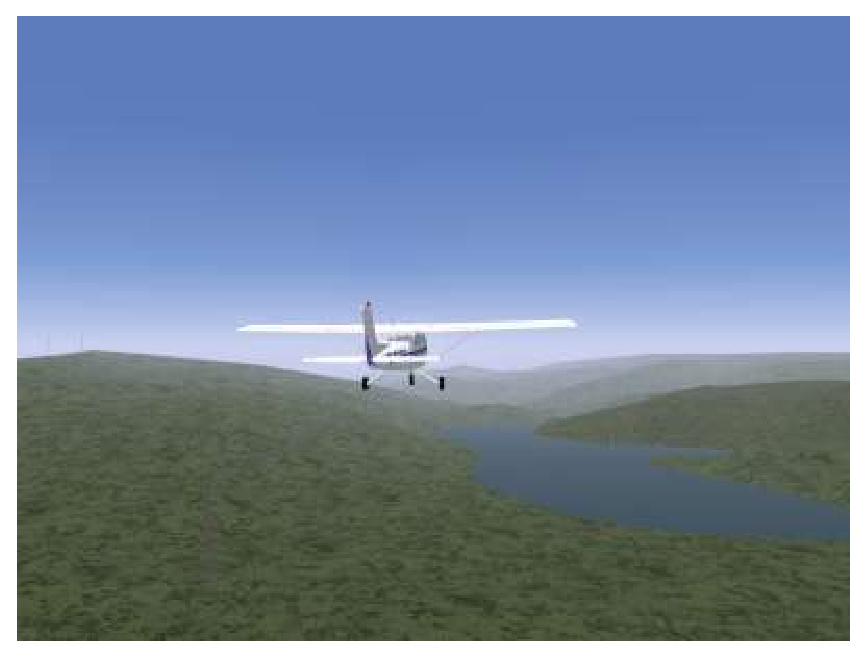
\includegraphics[width=0.5\textwidth]{calaveras1}
\caption{The Calaveras Reservoir}
\end{figure}

As we noted above, we're going to be travelling over a couple of reservoirs.
When you leveled off, the first (Calaveras) was probably right in front of you.
You can use them to check your position on the map. If it looks like you're
heading off course, twist the heading bug to compensate.

\subsection{Mixture}

\begin{figure}[!htp]
\centering
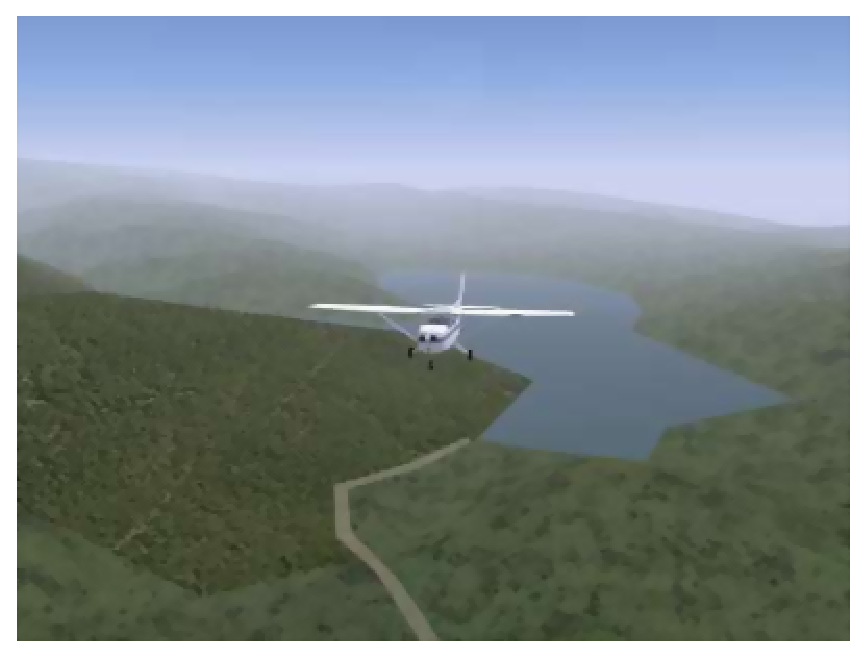
\includegraphics[width=0.5\textwidth]{calaveras2}
\caption{The Calaveras Reservoir}
\end{figure}

As altitude increases, the air gets thinner and contains less oxygen.
This means that less fuel can be burnt each engine cycle.
The engine in the C172 is simple and doesn't automatically
adjust the amount of fuel to compensate for this lack of oxygen.
This results in an inefficient fuel burn and a reduction in power
because the fuel-air mixture is too `rich'. We can control the
amount of fuel entering the engine every cycle using the \Index{mixture} control.
This is the red lever next to the throttle. By pulling it out, we `lean'
the mixture. We don't want the mixture too rich, nor too lean.
Both these conditions don't produce as much power as we'd like.
Nor do we want it perfect, because this causes the fuel-air to explode,
rather than burn in a controlled manner, which is a quick way to trash an engine.

\begin{figure}[!htp]
\centering
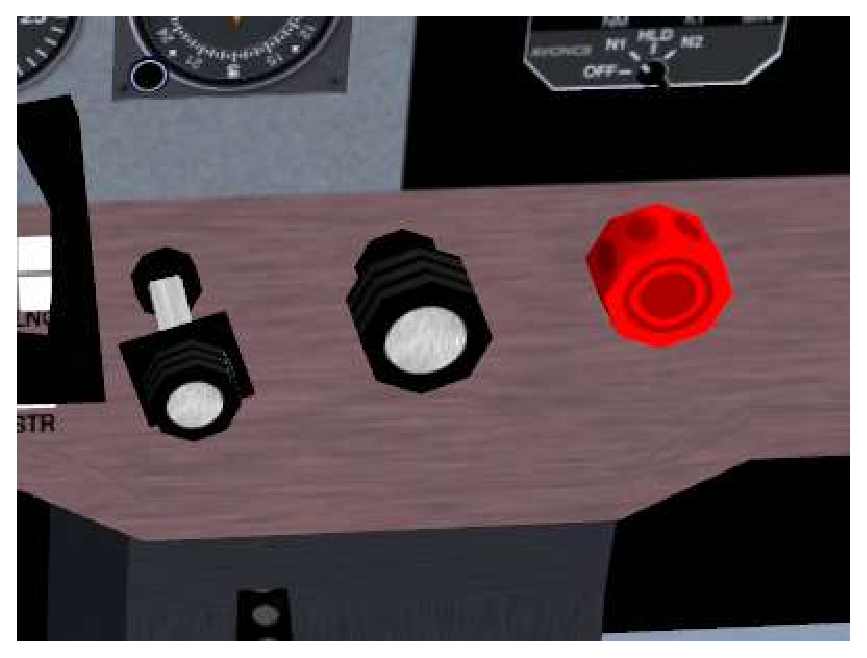
\includegraphics[width=0.5\textwidth]{mixture}
\caption{Mixture Control\label{mixture}}
\end{figure}

The mixture is controlled by the red lever to the right of the yoke.
You may need to pan your cockpit view to see it.

To pan the cockpit view, hold down the right mouse button Moving the mouse now
pans the view. Once you can see the mixture lever clearly, release the right
mouse button.

\begin{figure}[!htp]
\centering
\includegraphics[width=0.5\textwidth]{fuel_flow}
\caption{Fuel Flow and EGT guages\label{egt}}
\end{figure}

Pull the mixture lever out slowly (use Ctrl-C to see the hot spots),
leaning the mixture. As you do so, you'll see various engine instruments
(on the left of the panel) change. Fuel flow will go down (we're burning
less fuel), EGT (Exhaust Gas Temperature) will go up (we're getting closer
to a `perfect mixture') and RPM will increase (we're producing more power).
Pull the mixture lever out until you see the EGT go off the scale, then
push it in a bit. We're now running slightly rich of peak. While at
3,500ft we don't need to lean much, at higher altitudes leaning the
engine is critical for performance.

\section{Getting Down}

Once you reach the second reservoir (the San Antonio Reservoir),
we need to start planning our descent and landing at Livermore.
Landing is a lot more complicated than taking off, assuming you
want to get down in one piece, so you may want to pause the
simulator (press `p') while reading this.

\subsection{Air Traffic Control}

In the Real World, we'd have been in contact with \Index{Air Traffic Control} (ATC)
continually, as the bay area is quite congested in the air as well as on the ground.
ATC would probably provide us with a `flight following' service, and would continually
warn us about planes around us, helping to avoid any possible collisions.
The FlightGear skies are generally clear of traffic, so we don't need a flight following service.
If you want to change the amount of traffic in the sky, you can do so from the AI menu.

Livermore Airport is Towered (towered airports are drawn in blue on the sectional),
so we will need to communicate with the tower to receive instructions on how and where to land.

Before that, we should listen to the ATIS, and re-adjust our altimeter,
just in case anything has changed. This is quite unlikely on such a short flight,
but if flying hundreds of milesm it might make a difference. To save time when tuning
radios, you can access the Radio Settings dialog from the Equipment menu.
The Livermore ATIS frequency is 119.65MHz.

An ATIS message also has a phonetic letter (Alpha, Bravo, \ldots{} Zulu) to identify
the message. This phonetic is changed each time the recorded message is updated.
When first contacting a tower, the pilot mentions the identifier, so the tower can
double-check the pilot has up to date information.

Besides the altitude and weather information, the ATIS will also say which runway is in use.
This is useful for planning our landing. Normally, due to the prevalent Westerly wind,
Livermore has runways 25R and 25L in use.

Once you've got the ATIS, tune the radio to Livermore Tower. The frequency is 118.1MHz.
Depending on the level of AI traffic you have configured on your system, you may hear
Livermore Tower talking to other aircraft that are landing or departing.
This information is not played over the speakers, it is only displayed on the screen.

Once the frequency goes quiet, press the ' key. This will bring up the ATC menu.
Click on the radio button on the left to select what you wish to say (you only have one option), then OK.

Your transmission will be displayed at the top of the screen.
It will indicate who you are (type and tail number), where you are (e.g. 6 miles south),
that you are landing, and the ATIS you have.

After a couple of seconds, Livermore Tower will respond, addressing you by name and
telling you what runway to use, which pattern is in use and when to contact them, for example

\begin{quote}
``Golf Foxtrot Sierra, Livermore Tower, Report left downwind runway two five left.''
\end{quote}

To understand what this means, we'll have to describe the Traffic Pattern.

\subsection{The Traffic Pattern}

With the number of aircraft flying around, there have to be standard procedures
for take-off and landing, otherwise someone might try to land on-top of an aircraft taking off.

The \Index{Traffic Pattern} is a standard route all aircraft must follow when
near an airport, either taking off or landing. The traffic pattern has four
stages (or `legs'), shown in Figure~\ref{pattern}. The `downwind' mentioned
above refers to one of these, the one with the number 3.

\begin{figure}[!htp]
\centering
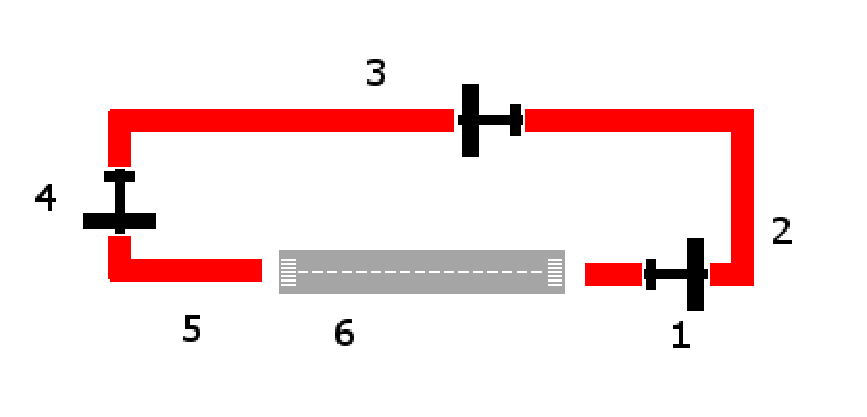
\includegraphics[width=0.5\textwidth]{pattern}
\caption{The Traffic Pattern\label{pattern}}
\end{figure}

\begin{enumerate}
\item Aircraft take off from the runway and climb. If they are leaving the
airport, they just continue climbing straight ahead until clear of the
pattern and then do whatever they like. If they are returning to the runway
(for example to practise landing), they continue climbing until they reach a
couple of hundred feet below `pattern altitude'. This varies from country to
country, but is usually between 500ft and 1000ft Above Ground Level (AGL).
This is called the \emph{upwind} leg.

\item The pilot makes a 90 degree left-hand turn onto the \emph{crosswind} leg.
They continue their climb to `pattern altitude' and level out.

\item After about 45 seconds to a minute on the crosswind leg,
the pilot again makes a 90 degree left turn onto the \emph{downwind} leg.
Aircraft arriving from other airports join the pattern at this point,
approaching from a 45 degree angle away from the runway.

\item When a mile or so past the end of the runway (a good guide is when the
runway is 45 degrees behind you), the pilot turns 90 degrees again onto the
\emph{base} leg and begins the descent to the runway, dropping flaps as appropriate.
A descent rate of about 500fpm is good.

\item After about 45 seconds the pilot turns again onto the \emph{final} leg.
It can be hard to estimate exactly when to perform this turn.
Final adjustments for landing are made.
I usually have to make small turns to align with the runway properly.

\item The aircraft lands. If the pilot is practising take-offs and landings,
full power can be applied and flaps retracted for takeoff, and the aircraft
can take off once more. This is known as `touch-and-go'.

\end{enumerate}

Most patterns at left-handed, i.e. all turns are to the left, as described
above. Right-hand patterns also exist, and are marked as `RP' on the sectional.
ATC will also advise you what pattern is in use.

\subsection{Approach}

\begin{figure}[!htp]
\centering
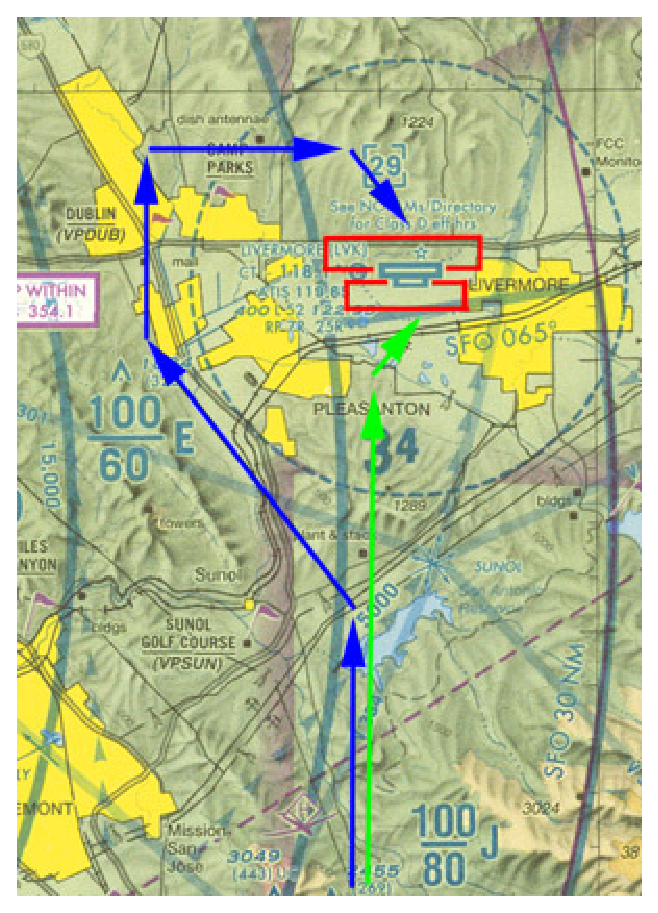
\includegraphics[width=0.5\textwidth]{livermore_pattern3}
\caption{Sectional extract showing approaches to Livermore\label{approach}}
\end{figure}

We're approaching Livermore airport from the South, while the runways run East/West.
Due to the prevailing Westerly wind, we'll usually be directed to either
runway 25R or 25L. 25R uses a right-hand pattern, while 25L uses a left-hand pattern.
Both the patterns are illustrated in Figure~\ref{approach}.
Depending on the runway we've been assigned, we'll approach the airport in one of two ways.
If we've been asked to land on runway 25R, we'll follow the blue line in the diagram.
If we've been asked to land on runway 25L, we'll follow the green line.

We also need to reduce our altitude. We want to end up joining the pattern at pattern
altitude, about 1,000ft above ground level (AGL). Livermore airport is at 400 ft above
sea-level (ASL), so we need to descend to an altitude of 1400 ASL.

We want to begin our maneuvers well before we reach the airport.
Otherwise we're likely to arrive too high, too fast, and probably
coming from the wrong direction. Not the best start for a perfect landing :).

So, let`s start descending immediately.

\begin{enumerate}
\item First switch off the autopilot by pressing the AP switch.

\item Return mixture to fully rich (pushed right in). If we were landing at a
high airport, we'd just enrich the mixture slightly and re-adjust when we reached the pattern.

\item Apply carb-heat. This stops ice forming when the fuel and air mix before
entering the cylinder, something that can often happen during descent in humid air.
The carb-heat lever is located between the throttle and mixture. Pull it out to apply heat.

\item Reduce power quite a bit. Otherwise we might stress the airframe due to over-speeding.

\item Drop the nose slightly to start the descent.

\item Trim the aircraft.

\end{enumerate}

Use your location relative to the airport and the two towns of Pleasanton and
Livermore to navigate yourself to the pattern following the general guide above.

Once you're established on the downwind leg, you'll need to report to ATC again.
Do this in the same way as before. They will then tell you where you are in the
queue to land. `Number 1' means there are no planes ahead of you, while
`Number 9' means you might want to go to a less busy airport! They'll also
tell you who is ahead of you and where. For example `Number 2 for landing,
follow the Cessna on short final' means that there is a single aircraft in
front of you that is currently on the final leg of the pattern. When they land and are
clear of the runway, they'll tell ATC, who can then tell you `Number 1 for landing'.

\subsection{VASI}

\begin{figure}[!htp]
\centering
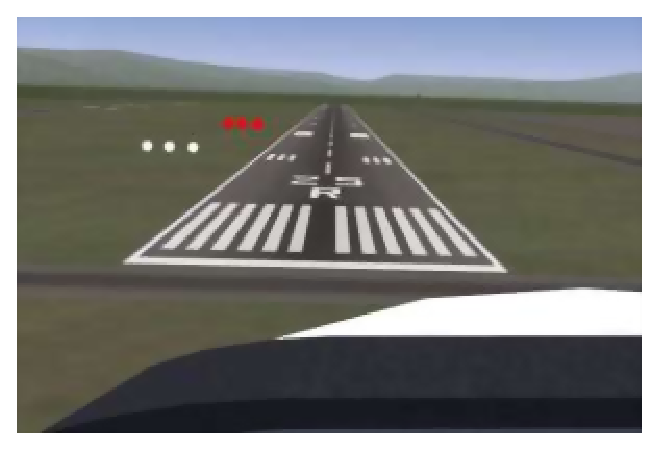
\includegraphics[width=0.5\textwidth]{vasi2}
\caption{On Final at Livermore with VASI on the left\label{vasi}}
\end{figure}

Once on final, you'll notice two sets of lights on the left of the runway
(enhanced in Figure~\ref{vasi}). This is the \Index{VASI} and provides a
nice visual clue as to whether you're too low or too high on approach.
Each set of lights can either be white or red. White means too high, red
means too low. White and red together means just perfect. On a Cessna
approaching at 60kts, a descent rate of about 500fpm should be fine.
If you are too high, just decrease power to increase your descent rate to
700fpm. If you are too low, increase power to decrease your descent rate to 200fpm.

\subsection{Go Around}

\begin{figure}[!htp]
\centering
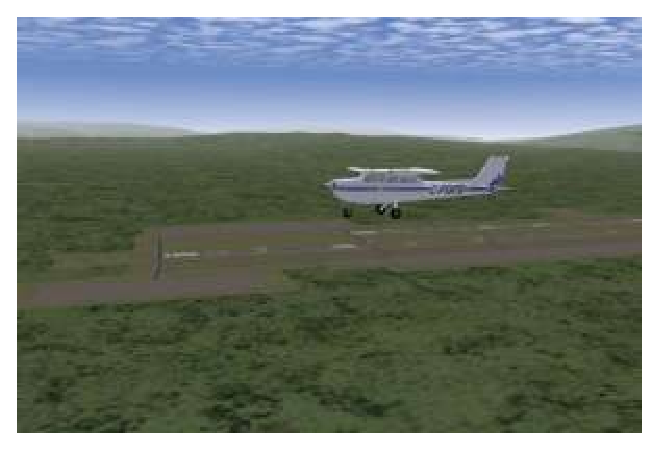
\includegraphics[width=0.5\textwidth]{missed}
\caption{Missed approach at Livermore}
\end{figure}

If for some reason it looks like you're going to mess up the landing
you can abort the landing and try again. This is called a `\Index{Go Around}'. To do this

\begin{enumerate}

\item Apply full power

\item Wait until you have a positive rate of climb - i.e.
your altitude is increasing according to the altimeter.

\item Raise your flaps to 10 degrees (first-stage).

\item Tell ATC you are `going around'

\item Climb to pattern height

\item If you aborted on final approach, continue over the runway to
re-join the pattern on the crosswind leg. If on base, fly past the
turn for final, then turn and fly parallel to the runway on the
opposite side from downwind to rejoin on the crosswind leg.

\item Fly the complete pattern, telling ATC when you are on downwind, and try again.

\end{enumerate}

\subsection{Clearing the Runway}

Once you're on the ground, you should taxi off the runway, then tell
ATC you are clear. At high-altitude airports, you would lean the engine to
avoid fouling the spark-plugs with an over-rich mixture.
Find somewhere nice to park, shut down the engine by pulling mixture to full lean,
then throttle off and magnetos to off (knob on the bottom left of the panel).
Switch off the avionics master switch, tie down the aircraft, then go get that hamburger!

I hope this tutorial is of some use. If you have any comments,
please let me know at stuart\_d\_buchanan \{at\} yahoo.co.uk.
\fi
